\begin{block}{Partitions interactives}
\begin{figure}
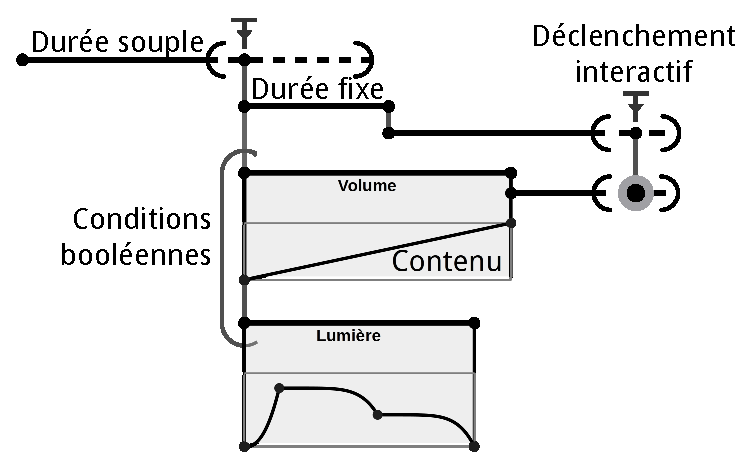
\includegraphics[width=\columnwidth]{images/score.eps}
\caption{Syntaxe d'une partition interactive}
\end{figure}
Autres approches:  Antescofo, INscore, OpenMusic, environnements de programmation (Tuiles réactives).

Application : musique, scénographie, contrôle de robots
\end{block}